% mainfile: ../../../../master.tex
\subsection{RNA quantification with NanoDrop}
% The part of the label after the colon must match the file name. Otherwise,
% conditional compilation based on task labels does NOT work.
\label{task:20180110_cj1}
\tags{qnt,rna,lab}
\authors{cj}
%\files{}
%\persons{}

\begin{figure}[H] % position of the figure 
    \centering
    \caption{Screenshots of the NanoDrop analysis of RNA samples extracted from liquid culture}
    \label{fig:CJ20180109}
    \begin{subfigure}[b]{0.49\textwidth}
        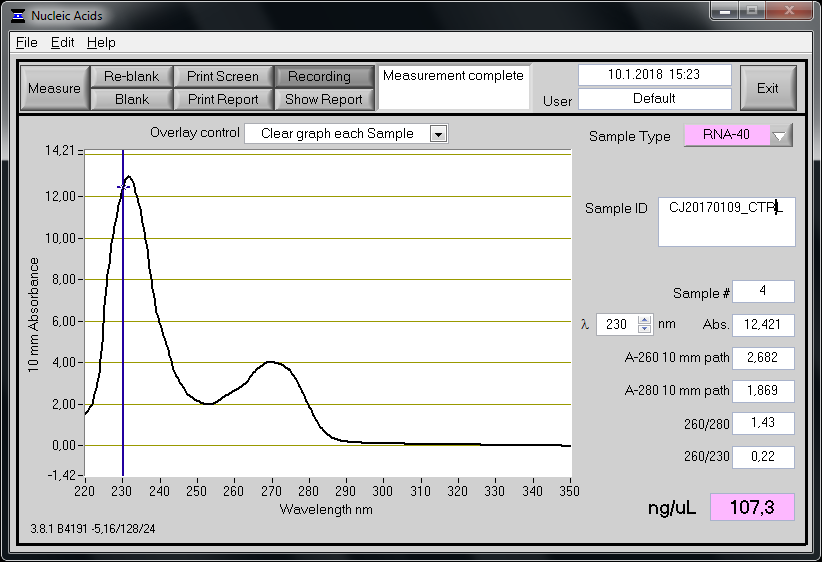
\includegraphics[width=\textwidth]{graphics/screenshots/CJ20180109_CTRL.png}
        \caption{Negative control of extraction}
        \label{sfig:CJ20180109_CTRL}
    \end{subfigure}
    ~ 
    \begin{subfigure}[b]{0.49\textwidth}
        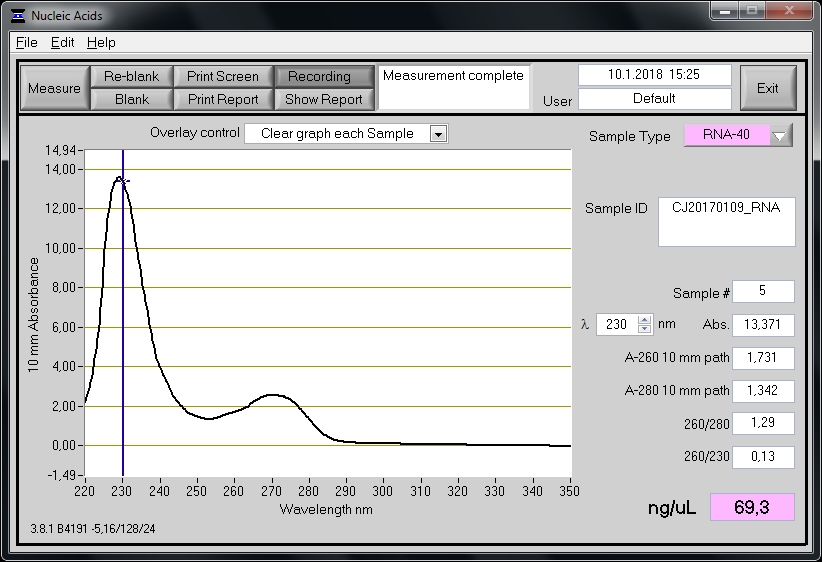
\includegraphics[width=\textwidth]{graphics/screenshots/CJ20180109_RNA.png}
        \caption{Extracted RNA sample}
        \label{sfig:CJ20180109_RNA}
    \end{subfigure}
\end{figure}

So the NanoDrop results are not as expected: according to the results shown in figure \ref{fig:CJ20180109}, my negative control has more RNA than my sample.

A 260/280 ratio of 2.0 is generally accepted as "pure" for RNA, here the ratios are too low (1.43 and 1.29 for \texttt{CTRL} and \texttt{RNA} respectively). Such low 260/280 ratios indicated the presence of contaminants.